% 1. Presentación del problema de infiltración de agua
% 1.1 Ventajas de la simulación % Arley ayuda, sin tantas ecuaciones.
% Optimizar el uso del agua en el suelo, lograr el mayor contacto entre las capas periféricas de la raíz del suelo. 1 gota de aceite contamina un litro de agua. riego por surco, problema del percolación, los nutrientes son llevados, ejemplo con el café tradicional. problema
% cantidad desmedida de agua porque el suelo pierde sus nutrientes, %60% de eficiencia
% ejemplo de la caña: pesticidas, exceso de agua, etc (ciclo).
% el perder agua es mucho más caro para la humanidad.
% aportar a la agricultura de precisión
% ruta apoplástica (explica la interacción de la raíz agua)
% % el efecto de las algas (dia/noche) se puede explicar con el cloropasto () y la mitocondria (respiración)
% qué solución hay.
% de lo general a particular.
% [1] Ref.
\section{Presentation of water infiltration problem}
% \subsection{Importancia}
% \subsection{Justificación}
% \subsection{Descripción del problema}
\subsection{Ecological footprint of the water cycle on agriculture}

\begin{frame}
	\frametitle{\subsecname}
	\begin{figure}[ht!]
		\centering
		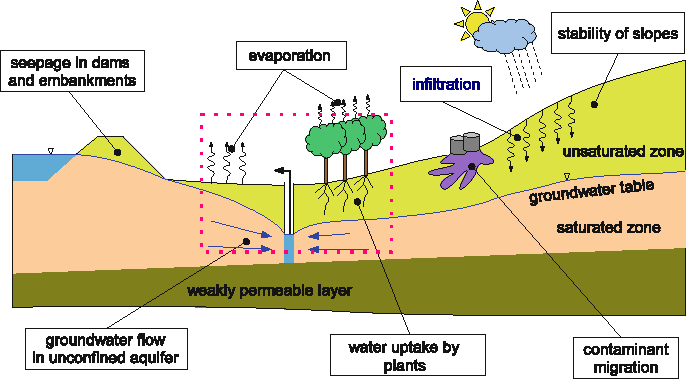
\includegraphics[height=7cm]{contamination}
	\end{figure}
	\note{
		En la diapositiva se muestra una de estas situaciones diarias.

		También se tiene un anexo donde se estudia un software libre
		como es \lstinline|wxmaxima|.
	}
\end{frame}
% TODO: Poner la imagen en el centro, y en ovalos redondeados colocar las ideas del primer p'arrafo
% TODO: es decir, crecimiento poblacional, demanda de alimentos
% TODO: Agricultura que no es de precision, agua.
% https://tex.stackexchange.com/questions/96289/how-to-connect-beamer-blocks-by-arrows
% \subsection{Problem}
\begin{frame}
	\frametitle{\secname}
	\begin{minipage}{0.6\textwidth}
		\begin{itemize}
			\item
				  Population and urban growth for years, has increased 
				  both the demand for food and the exploitation of resources
				  such as water and soil for agricultural activities. However, in an 
				  effort to satisfy the demand, we have neglected good management 
				  and stability of the surronunding ecosystems. \cite{Latham1997}
			      % El desarrollo urbano, en conjunto con el crecimiento poblacional
			      % a lo largo de los años, ha llevado al alza de la demanda de
			      % alimentos por parte del ser humano, motivo por el cual se se a
			      % visto en la obligación explotar cada vez más los recursos naturales que lo rodean y utilizar más terrenos para diversas actividades agrarias, sin embargo en su afán de suplir dicha demanda ha descuidado el buen manejo de los recursos naturales y la estabilidad de los ecosistemas que lo rodean.

			\item

			One of the main problems with the greatest environmental 
			impact is the inefficient use of water management when 
			implementing irrigation systems. As a consequence, 
			large amounts of water are consumed, groundwater levels are 
			polluted, affecting the water footprint, and soils deteriorate.

			\textbf{Soil is a non-renewable resource!!!}.
			      % Actualmente en la agricultura uno de los problemas más frecuentes  y de mayor impacto ambiental que genera el mal manejo de los cultivos, es el uso ineficiente de los recursos hídricos, al implementar sistemas de riego poco eficaces, al tratar satisfacer la demanda hídrica que generan las plantas. Además es uno de los puntos más importantes que se abordan en temas ambientales y que no solo preocupa por el desperdicio de agua sino también por el daño y las pérdidas que puede ocasionar en las propiedades fisicoquímicas del suelo.
			      % https://proain.com/blogs/notas-tecnicas/calidad-del-agua-para-riego-agricola
		\end{itemize}
	\end{minipage}
	\begin{minipage}{0.37\textwidth}
		\begin{figure}[ht!]
			\centering
			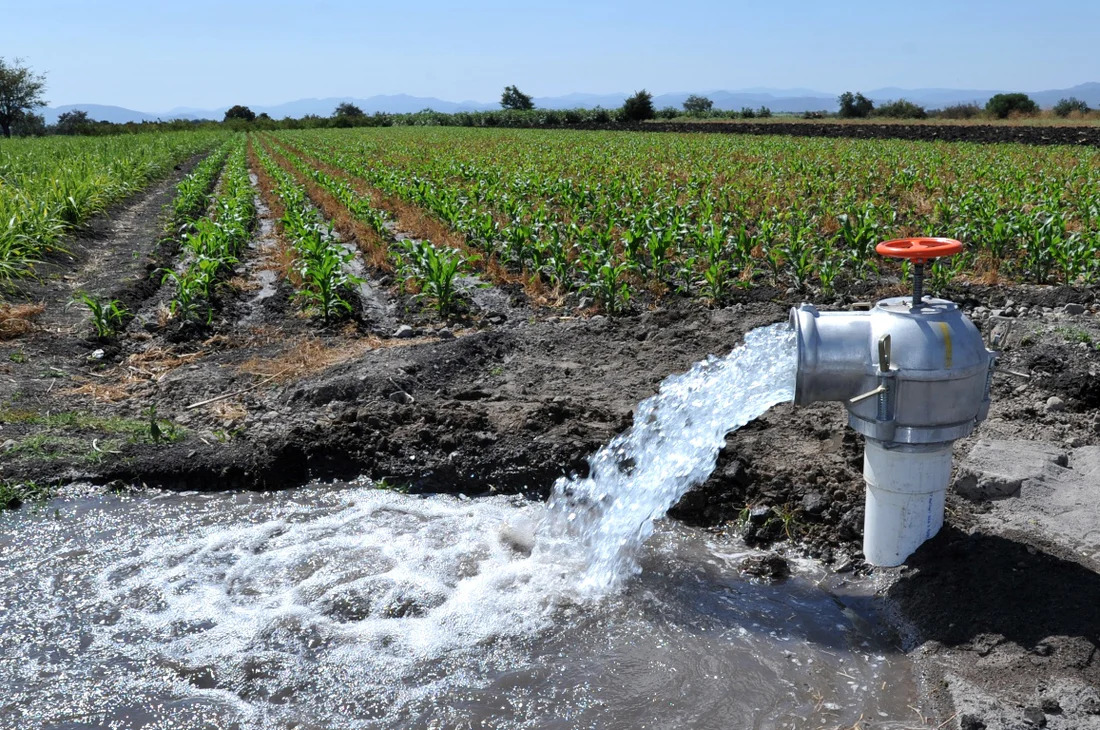
\includegraphics[height=4cm]{wasted_water}
		\end{figure}
	\end{minipage}
\end{frame}

\begin{frame}
	\frametitle{\secname}
	\begin{minipage}{0.5\textwidth}
		\begin{itemize}
			\item In Valle del Cauca, for example, one of the most 
			common crops is sugar cane, which generates contamination 
			problems for both the soil and groundwater (aquifers).
			\item Currently, these aquifers supply more than 80\% 
			of the useful water used throughout the region, 
			and the impacts of fertilizers and inefficient irrigation 
			systems that currently exist are unknown.

		\end{itemize}
	\end{minipage}
	\begin{minipage}{0.47\textwidth}
		\begin{figure}[ht!]
			\centering
			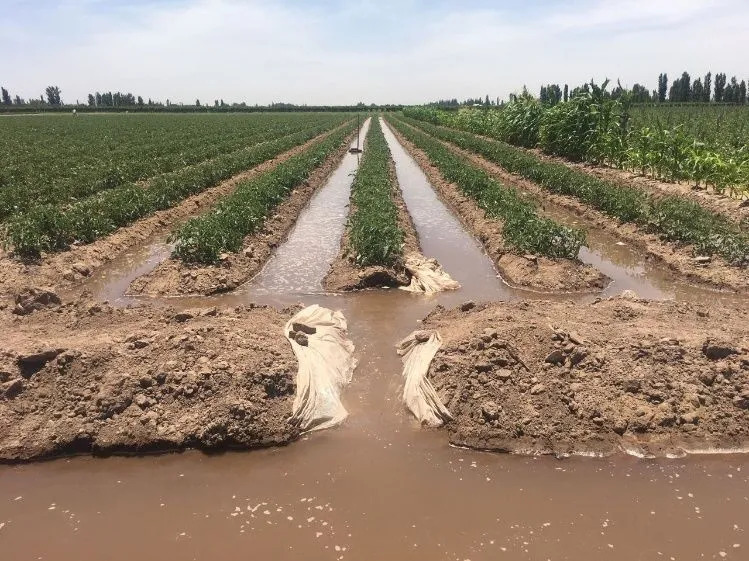
\includegraphics[height=5.5cm]{water_waster2}
			% https://www.agromeat.com/284499/conceptos-tecnicas-y-estrategias-en-uso-eficiente-del-agua-de-riego
		\end{figure}
	\end{minipage}
\end{frame}
% Irricad
\section{Advantage of a Simulation}
\begin{frame}
	\frametitle{\secname}
	%\begin{minipage}{0.5\textwidth}
		\begin{itemize}
			\item The objective is to optimize the use of water in 
			agricultural activities, including mathematical modelling. 
			The purpose is to study the Richard's equation and simulate 
			the behavior in the water-soil interaction, trying to deepen 
			the understanding of the infiltration phenomenon.
			\item It also saves time and money, since several variables 
			and conditions of interest, such as temperature, humidity, 
			saturation, etc., can be included prior to field testing.
			\item The simulation also allows studying various types of 
			soil and different interactions, for example with organic 
			matter, plants, nutrients, etc. These studies will allow the 
			improvement of different plant species and agricultural methods.
			\item It is also necessary to study how and for how long 
			contaminants infiltrate the soil and reach the aquifers.
		\end{itemize}
	%\end{minipage}
	%\begin{minipage}{0.47\textwidth}
	%	\begin{figure}[ht!]
	%		\centering
	%		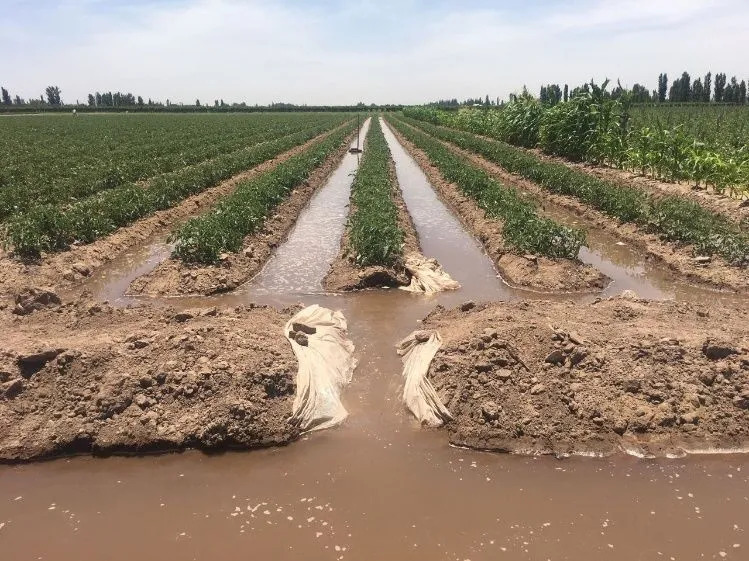
\includegraphics[height=5.5cm]{water_waster2}
			% https://www.agromeat.com/284499/conceptos-tecnicas-y-estrategias-en-uso-eficiente-del-agua-de-riego
	%	\end{figure}
	%\end{minipage}
\end{frame}
\section{The soil and his features}
\begin{frame}
	\frametitle{\secname}
	Soils have different properties, physical, mechanical, electrical, 
	among others. They also have different pore sizes, and thus are 
	classified, for which the textural triangle is used.
	Not all soils are the same, nor are they used for the same purposes, 
	so soil studies must be carried out to determine their characteristics 
	and properties.
	\begin{figure}[ht!]
		\centering
		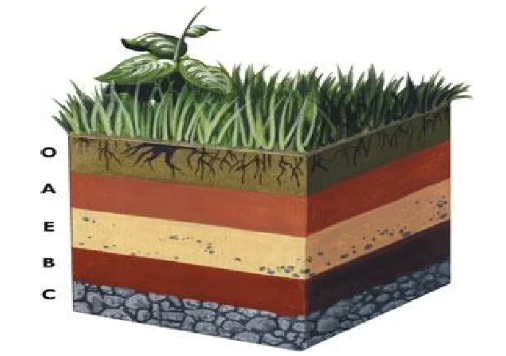
\includegraphics[height=5.5cm]{propiedades-suelo}
	\end{figure}
\end{frame}
\begin{frame}
	\frametitle{\secname}
	\begin{minipage}{0.47\textwidth}
		\begin{figure}[ht!]
			\centering
			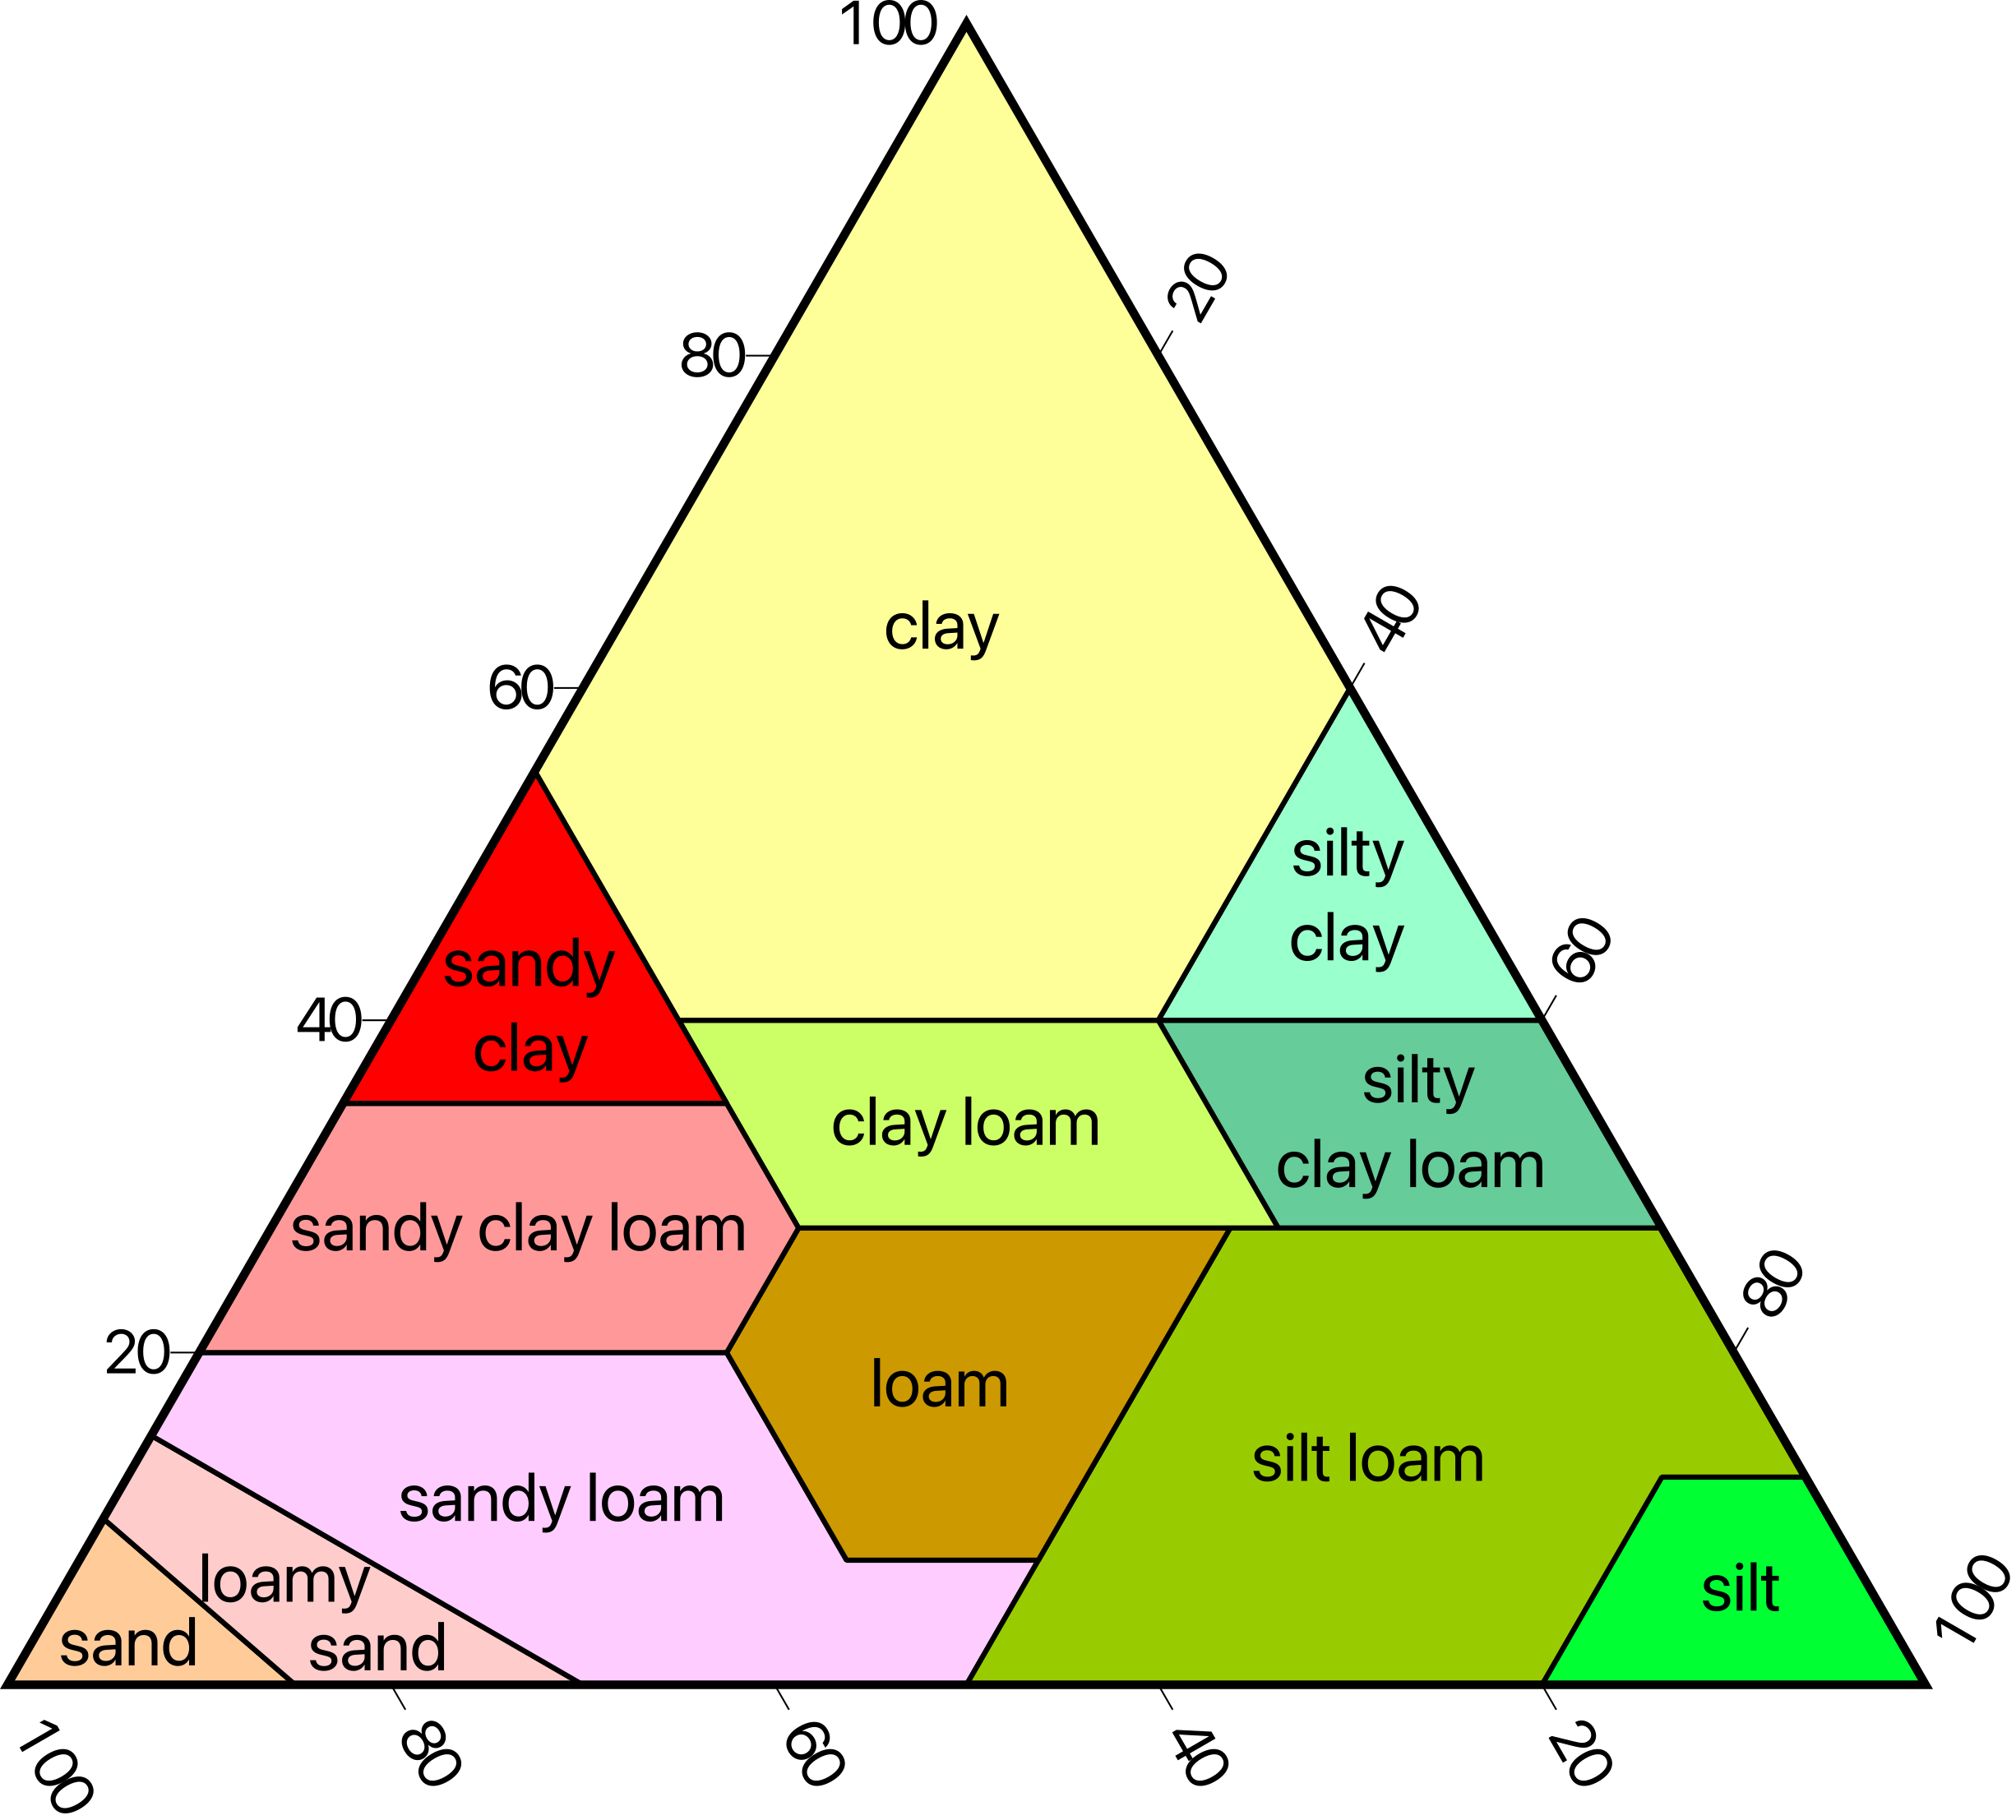
\includegraphics[height=5.5cm]{textural_soil}
		\end{figure}
	\end{minipage}
	\begin{minipage}{0.5\textwidth}
		\lstinputlisting[
			caption={Spatial parameters \texttt{soil.params}.},
			label=soil.params,
		]{../../../script/soil.params}
	\end{minipage}
\end{frame}
\section{Soil water content} % Humedad en el suelo
\begin{frame}
	\frametitle{\secname}
	Depending on the porosity and characteristics, soils can retain water in different ways, the amount of water that cannot be easily obtained is called residual water, when there is a little more water, it is called permanent wilting point because the plants cannot yet dispose of that water, it is strongly trapped by the pores.

When the soil has water available to the plant, but still has empty air spaces, it is called field capacity. And finally, when it is completely filled with water, the soil is said to be saturated.

\end{frame}
\begin{frame}
	\frametitle{\secname}
	\begin{figure}[ht!]
		\centering
		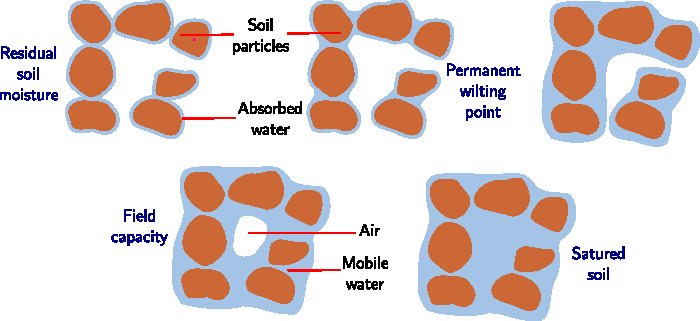
\includegraphics[height=6.8cm]{wetness}
	\end{figure}
\end{frame}
% https://i.pinimg.com/originals/34/66/77/34667762422298ffc10fec5252f28619.jpg

\section{Capillarity}

\begin{frame}
	\frametitle{\secname}
	\begin{center}\Huge % TODO: Poner sobre un fondo con relleno sin bordes.
		\fbox{What is the capillarity water soil?}
	\end{center}
\end{frame}
\begin{frame}
	\frametitle{\secname}
	Capillarity is a property of liquids that depends on their surface tension, which, in turn, depends on the cohesion of the liquid, and which gives it the ability to move up or down a capillary tube.

When a liquid moves up a capillary tube, it is because the intermolecular force or intermolecular cohesion is less than the adhesion of the liquid to the tube material; that is, it is a wetting liquid. The liquid continues to rise until the surface tension is balanced by the weight of the liquid filling the tube. This is the case of water, and it is this property that partially regulates its ascent within plants, without expending energy to overcome gravity.
\end{frame}

\begin{frame}
	\frametitle{\secname}
	\begin{minipage}{0.5\textwidth}
		\begin{align*}
			\Delta p=p_{\mathrm{a}}-p_{\mathrm{w}} & =
			\sigma_{\mathrm{aw}}\left(\frac{1}{r_{\mathrm{c} 1}}+\frac{1}{r_{\mathrm{c} 2}}\right)
			=\frac{2 \sigma_{\mathrm{aw}} \cos \psi}{r_{\mathrm{c}}}                                  \\[\baselineskip]
			\sigma_{\mathrm{aw}}\cos\psi           & =\sigma_{\mathrm{Sa}}-\sigma_{\mathrm{Sw}},\quad
			h_{\mathrm{c}} =\frac{1.5 \times 10^{-5}}{r_{\mathrm{c}}}
		\end{align*}
		\begin{itemize}
			\item $\sigma_{\mathrm{aw}}$ is the surface tension of the air-water interface.
			\item $\sigma_{\mathrm{Sa}}$ is the surface tension of the solid-air interface.
			\item $\sigma_{\mathrm{Sw}}$ is the surface tension of the solid-water interface.
			\item $\psi$ is the wetting angle.
		\end{itemize}
	\end{minipage}
	\begin{minipage}{0.47\textwidth}
		\begin{figure}[ht!]
			\centering
			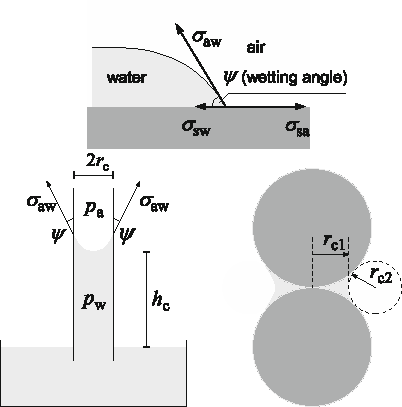
\includegraphics[height=6.2cm]{capillar_preassure}
		\end{figure}
	\end{minipage}
\end{frame}

